\chapter{\hlc[red]{Discussion \& Conclusion}} \label{ch:conclusion}

\section{\hlc[red]{Summary and Contributions}}

\subsection{\hlc[red]{Theory \& Critical Analysis}}

\subsection{\hlc[red]{The EVDT Framework}}

\subsection{\hlc[red]{Rio de Janeiro Development \& Mangroves}}

\subsection{\hlc[red]{Vida Decision Support System for COVID-19 Response}}

\section{\hlc[red]{Opportunities for Future Inquiry}}

Research Question 3: ``What steps are necessary to establish \ac{evdt} as a continually development framework, a community of practice, and a growing code repository?"

Research Deliverable 3a: ``An assessment of lessons learned from these \ac{dss} development processes"

Research Deliverable 3b: ``An outline of potential future \ac{evdt} refinement and extension, such as using \ac{evdt} to inform the development of future \ac{eo} systems that are better designed for particular application contexts"

Chapter \ref{ch:conclusion} will review these lessons, including discussing how the case studies would have been performed differently in retrospect.

The second portion of the chapter, Section \ref{sec:critiques}, turns towards to critiques of the literature and the concept of this thesis. It is an attempt to recognize and preemptively address potential pitfalls of the approach taken in this thesis. These are primarily fundamental or ethical concerns, as opposed to mere questions of implementation, the latter of which are largely held for Chapter \ref{ch:conclusion}.

\subsection{\hlc[red]{In Rio de Janeiro \& Mangroves Globally}}

\subsection{\hlc[red]{Lessons from COVID-19}}

\subsection{\hlc[red]{The Future of EVDT}} \label{sec:future}


[** discuss evdt with regard to EO value chain]

\begin{figure}[h]
\centering
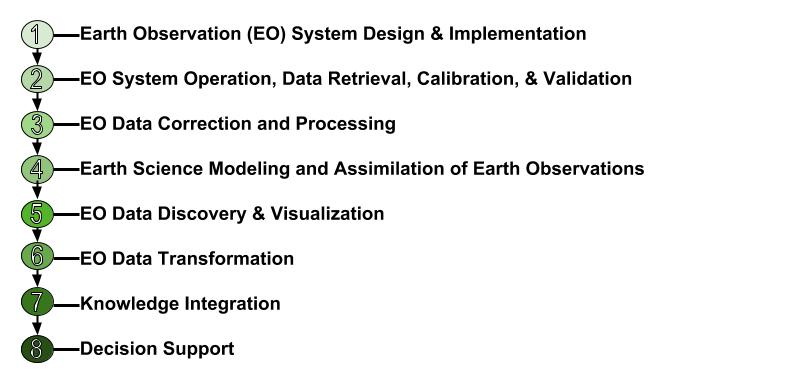
\includegraphics[width=0.9\textwidth]{Figures/chap6/EOChain.jpg}
\caption[Generic Earth Observation Data Value Chain]{Generic Earth Observation Data Value Chain}
\label{fig:eochain}
\end{figure}

the potential of EVDT beyond this thesis 

EVDT is broadly applicable, not just for small geographic projects. Flexible and adaptable.
 (space sustainability)
 


There are certain key design requirements that this team has identified for the development of \ac{evdt} applications. Some of these are listed here.

\textit{Rapid Prototyping \& Co-Design:} In order to confirm that the proper data and dynamics are being captured, as well as to ensure the utility of the model to decision-makers and designers, the key stakeholders must be involved at all stages of the design process. Additionally, since most individuals have a difficult time providing concrete advice and criticism when discussing the abstract, rapid prototyping and mock-ups are important for stimulating feedback. One key component of this is always making sure that the user interface is available in the native language of the primary users.

\textit{Enlist appropriate experts:} The design of any \ac{eos} is inherently interdisciplinary and this is also true for \ac{eo} applications. For this reason the development necessarily involves a wide range of collaborators who vary both in terms of discipline (systems engineering, earth science, economics, etc.) and it terms of institution (academic researchers, government officials, \ac{ngo} and corporate leaders, local activists, etc.). Rather than make assumptions when confronted with an issue outside our expertise, we do our utmost to recruit or consult with a relevant expert. Obviously such a large and diverse team is not feasible for every application nor does it scale particularly well. This is why the next requirement is present.

\textit{Open Access and Modularity for Adaptation and Reuse:} The intent is not for this team to develop complete, black-box products, but rather to facilitate the the tool development process for others. Part of this includes the co-design requirement, but another part is making the code itself readily available online and designing the implementation of the framework to be as reusable as possible. In this way, local government officials may be able to reuse previous \ac{eo} data processing techniques, while focusing on the vulnerability or decision-making components. This is also important to provide clarity on ultimate ownership and responsibility for the product.

\textit{Ensure computational accessibility:} Cloud-based and internet-hosted tools eliminate the need to direct possession of high performance computing equipment by either the end users or the developers. This reduces cost-of-entry for potential developers of \ac{evdt} models and ensures that end users can interact with, critique, and apply the models wherever they are, provided they have internet access. That is why our processing techniques and code either are hosted online or are designed to be able to run on a standard work laptop.

% Discuss different stakeholder interests and needs

\textit{Awareness of different stakeholder needs and interests:} While specific examples are discussed in the earlier sections, collaborators and users have a variety of educational backgrounds and personal priorities. This vary not only across institutions (such as government officials and local activists having different priorities) but also within an institution (such as an urban planning official assigned to a particular neighborhood versus one responsible for city macroplanning). We are often not aware of all of these differences, nor of pre-existing relationships and dynamics. For this reason it is important to cultivate relationships with a variety of local stakeholders, rather than relying on just on point of contact. The "outside expert" dynamic is also one prone to unintended consequences \cite{easterly2015}, which is why our team focuses on providing useful tools and insights, rather than on making concrete recommendations.




\section{\hlc[red]{Advancing Stakeholder-Informed Sustainable Development Decision-making}}


